\documentclass[a4paper,twoside,10pt]{article}
\usepackage{a4wide,graphicx,fancyhdr,amsmath,amssymb}
\usepackage{algorithm}
\usepackage{algorithmic}
\usepackage{hyperref}
\usepackage{ragged2e}

%----------------------- Macros and Definitions --------------------------

\setlength\headheight{20pt}
\addtolength\topmargin{-10pt}
\addtolength\footskip{20pt}

\newcommand{\N}{\mathbb{N}}
\newcommand{\ch}{\mathcal{CH}}

\newcommand{\exercise}[2]{\noindent{\bf Question #1 (#2pt):} \\\\ }

\fancypagestyle{plain}{%
\fancyhf{}
\fancyhead[LO,RE]{\sffamily\bfseries\large Eindhoven University of Technology}
\fancyhead[RO,LE]{\sffamily\bfseries\large 2IMM10 Recommender Systems}
\fancyfoot[LO,RE]{\sffamily\bfseries\large Department of Mathematics and Computer Science}
\fancyfoot[RO,LE]{\sffamily\bfseries\thepage}
\renewcommand{\headrulewidth}{0pt}
\renewcommand{\footrulewidth}{0pt}
}

\pagestyle{fancy}
\fancyhf{}
\fancyhead[RO,LE]{\sffamily\bfseries\large Eindhoven University of Technology}
\fancyhead[LO,RE]{\sffamily\bfseries\large 2IMM10 Recommender Systems}
\fancyfoot[LO,RE]{\sffamily\bfseries\large Department of Mathematics and Computer Science}
\fancyfoot[RO,LE]{\sffamily\bfseries\thepage}
\renewcommand{\headrulewidth}{1pt}
\renewcommand{\footrulewidth}{0pt}

%-------------------------------- Title ----------------------------------

\title{\vspace{-\baselineskip}\sffamily\bfseries Assignment XX \\
\large Deadline: tba}
%\author{Puck Mulders \qquad Student number: 0737709 \\{\tt p.j.a.m.mulders@student.tue.nl}}

\date{\today}

%--------------------------------- Text ----------------------------------

\begin{document}
\maketitle

\section*{Emojifier -- Classifying emotions with RNN (-pt)}

Sentiment analysis allows computer to identify human emotions from raw text information. Traditional approach mainly relies on count-based algorithm, i.e. by counting \textit{happy} or \textit{sad} words in observed text, and external knowledge base sentiment corpus (wordNet, sentiNet) -- as compared to neural-based methods we study in this course. 

\justify
Through Practicals 5-6 and Assignment 3 of the course, you have learned how to construct a Recurrent Neural Networks (RNN) model for a binary "Sentiment Classification" task.  This RNN model is used as an end-to-end application to detect sentiment polarity of text reviews, i.e. whether a statement can be categorized as \textit{positive} or \textit{negative} sentiment.

\justify
Instead of detecting sentiment polarity (positive or negative), you will build a RNN model for classifying human emotions in a more expressive message, i.e. by using emojis. Emoji is a graphical symbol (ideogram) of human's feelings, moods, and emotions -- which is mostly available in social network platforms, website, and mobile phone applications. Using the constructed model, you can express text with its predicted emoji label. You can further create an emoji sentiment score based on emotions found in corpus - or - you can use available emoji sentiment ranking to classify and analyse the sentiment polarity of text input. An advanced work \footnote{https://github.com/tlkh/text-emotion-classification} further utilizes this sentiment spectrum of emotions to detect fake news or illegitimate reviews.

\justify
In this assignment, you need to complete the following tasks:

\begin{enumerate}
    \item Preprocess data into training, validation, and test set, including creating the word vocabulary index and functions to transform raw emotion labels into numerical vectors and emojis. Briefly discuss the statistics of raw data (the statistical occurrences of emotion labels in observed corpus). 
    \item Construct a model to transform text input into ideograms (emoji) symbolizing emotions or moods of the corresponding text. Train and validate the model. Discuss the model performance during training and validation stage.
    \item Compute evaluation metrics: Confusion matrix, Accuracy, Precision, Recall, and F1-score from data set 1 (test set of "emotion" data).
    \item Discuss type of emotions in which the model is under-performed and its possible reasons. Give a running examples (i.e. text input and expected emoji vs. predicted emoji)
    \item Create a prototype of emoji sentiment ranking from data set 2 ("sentiment labelled sentences" data).
    
\end{enumerate}
\newpage
\subsection*{Data description}

\begin{enumerate}
    \item Twitter emotion sentiment \footnote{https://github.com/tlkh/text-emotion-classification}, can be downloaded from \url{https://storage.googleapis.com/trl_data/emotion.zip}. This twitter data set contains 40.000 raw tweets and its emotion labels (13 labels). Use this data for training, validating, and testing the constructed model. Choose a reasonable partition number to split the data.
    
    Note: You can use preprocessing code for twitter data, as in Practical 5.3 and 5.4. You will also need to transform 13 classes into 5 classes as a comparison task to analyse model performance. 
    
    \item Sentiment labelled sentences \footnote{https://archive.ics.uci.edu/ml/datasets/Sentiment+Labelled+Sentences}, i.e. sentences labelled as positive and negative, extracted from Amazon reviews, IMDB reviews, and Yelp. Each consists of 500 positive and 500 negative sentences. Data can be downloaded from \url{https://storage.googleapis.com/trl_data/sentiment_sentences.zip}. Use this data for the last task, creating a prototype of emoji sentiment ranking.
    
    \item Glove pretrained embedding from twitter data set, can be downloaded from \url{https://nlp.stanford.edu/projects/glove/}. Use this pretrained embedding as non-trainable weights for embedding layer in the constructed model.
    
\end{enumerate}

\subsection*{Model architecture}

Build emojifier - a two-layers RNN model based on the following architecture (Figure \ref{fig:rnnmodel}). You can either choose to use LSTM/GRU layer. Justify your chosen model architecture.

\begin{figure}[ht]
\centering
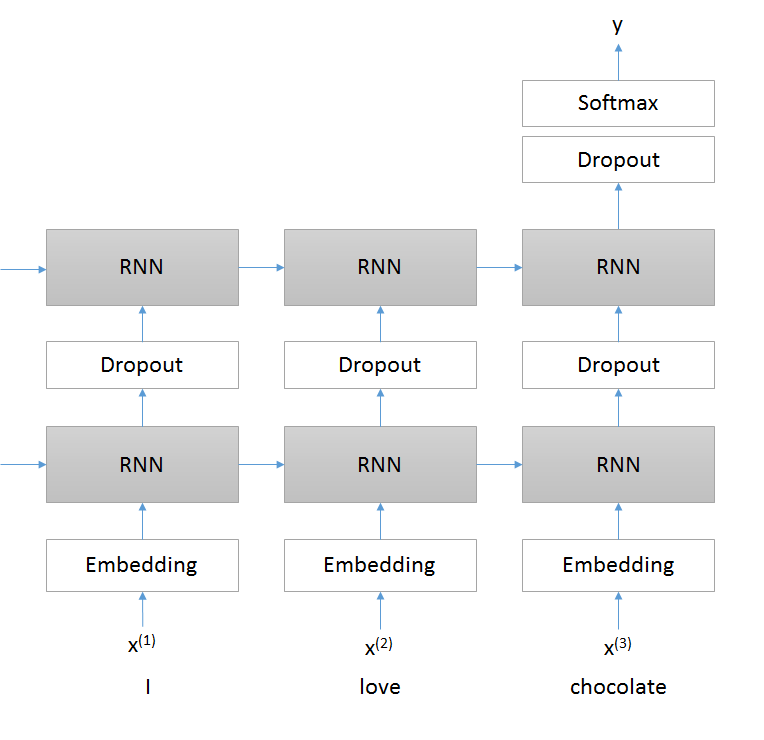
\includegraphics[scale=.6]{figures/model.png}
\caption{Emojifier - Two layers RNN Sequence Classifier}
\label{fig:rnnmodel}
\end{figure}  

\subsection*{Evaluation metrics}

Compute evaluation metrics (i.e. Accuracy, Precision, Recall, F1-Score) on two (2) preprocessed data, i.e. original data with 13 classes, and data with 5 classes to analyse model performance on two (2) settings of multi-class classification training and evaluation.

\justify
Note: This requires you to train the model on data with 5 classes as well. 

\subsection*{Sentiment spectrum of emotions/emojis}

\justify
Create a prototype of emoji sentiment ranking, as exemplified in \url{http://kt.ijs.si/data/Emoji_sentiment_ranking/} from "sentiment labelled sentences" data set.

\begin{itemize}
    \item Predict emotion labels (13 classes) of corresponding data sets (Amazon, IMDB, Yelp) using the model trained on twitter emotion data.
    \item Assuming your model prediction is nearly accurate (you do not have gold standard of "emotion labels" in this data set - and thus, we refer this as \textit{a prototype}), use the results (predicted emotion labels / emojis) to calculate the occurrences of each emotion label in positive and negative sentiments. Use the statistics to compute sentiment spectrum (percentage score) of each emoji / emotion label.    
\end{itemize}

\justify
Note: You do not need to create similar statistics. Use your own table presentation. The required information need to be present: emojis, emotion labels (text), total occurrences, positive occurrences, negative occurrences, sentiment bar/spectrum. 

\end{document}